
\فصل{مفاهیم اولیه}

بخش مفاهیم پایه، شامل کلیه مفاهیم اولیه‌ی مورد نیاز در ارتباط با این پژوهش می‌باشد. این بخش ابتدا تعاریف و توضیحاتی در رابطه با حریم خصوصی تفاضلی ارائه می‌دهد. سپس به بیان سازوکار‌های مرتبط با حفظ حریم خصوصی پرداخته می‌شود. در نهایت برخی از چالش‌های اساسی که پیش روی سازوکارهای حفظ حریم خصوصی هستند، بیان خواهد شد.  

\قسمت{حریم خصوصی تفاضلی}

حریم خصوصی تفاضلی یک چارچوب ریاضی است که تضمین می‌کند خروجی هر تحلیل آماری به‌گونه‌ای ساخته شود که حضور یا عدم حضورِ هر فرد در داده‌ها تأثیر محسوسی بر توزیع نتایج نگذارد. به بیان دیگر، حریم خصوصی تفاضلی این اجازه را می‌دهد که بتوان روی یک مجموعه داده، تحلیل‌های آماری مانند میانگین و شمارش را انجام دهیم ولی نتوان اطلاعات مربوط به یک شخص را استخراج کرد.
فرض کنید سازمانی می‌خواهد یک آمار تقریبی از تعداد افراد با یک بیماری خاص بدست‌آورد. این سازمان از تمام جامعه‌ی آماری خود درخواست می‌کند که با تکمیل فرمی بگویند آیا آن بیماری خاص را دارند یا خیر. همگی فرم‌ها به سمت سازمان فرستاده می‌شود. سپس سازمان باید نتایج را با کاربران خود به اشتراک بگذارد. اگر نتایج به دور از هیچگونه سازوکار امنیتی منتشر شود، حریم خصوصی افراد شرکت کننده در رابطه با داشتن بیماری خاص نقض می‌شود. نوعی از الگوریتم‌های حفظ حریم خصوصی، الگوریتم‌های حریم خصوصی تفاضی هستند که با ایجاد نوفه در داده‌ها، باعث می‌شوند  نتایج تحلیل‌های آماری به طوری تقریبی صحیح بوده و در عین حال، حریم خصوصی افراد حفظ شود.

تعریف حریم خصوصی تفاضلی برای اولین بار توسط خانم دُرک \مرجع{dwork2006our} به صورت زیر مطرح شد:

\شروع{تعریف}[حریم خصوصی تفاضلی]
الگوریتم $M$ را در نظر بگیرید که به عنوان ورودی پایگاه داده $D$ را دریافت می‌کند. این الگوریتم حریم خصوصی تفاضلی را در صورتی تضمین می‌کند که برای هر دو پایگاه داده مجاور $D$ و $D'$ و برای هر مجموعه خروجی $S$ ممکن داشته باشیم:

\begin{equation}
\Pr[\mathcal{M}(D) \in S] \leq e^\epsilon \times \Pr[\mathcal{M}(D') \in S]
\end{equation}

\برچسب{تعریف: حریم خصوصی تفاضلی}
\پایان{تعریف}

پایگاه داده‌هایی که تنها در یک عنصر تفاوت داشته باشند ، مجاور یا همسایه\پانویس{Neighbour} نامیده می‌شوند. همچنین $\epsilon$ یک ورودی مثبت با مقدار کم است و سطح حریم خصوصی را نشان می‌دهد. بنابر عبارت بالا، هر چه مقدار کمتری برای  $\epsilon$ در نظر بگیریم، در واقع قوانین سخت‌گیرانه‌تری برای حفظ حریم خصوصی اعمال کرده‌ایم.

\قسمت{بودجه حریم خصوصی}

بودجه حریم خصوصی یکی از مفاهیم کلیدی در حریم خصوصی تفاضلی است که برای اندازه‌گیری و کنترل میزان حریم خصوصی در طی اجرای یک الگوریتم یا مجموعه‌ای از الگوریتم‌ها استفاده می‌شود. این مفهوم به‌طور مستقیم با پارامتر $\epsilon$ در ارتباط است.

معمولا بودجه‌ای که برای الگوریتم‌های حافظ حریم خصوصی در نظر می‌گیرند، برابر 1 یا مقداری نزدیک به 1 است. هرچه بودجه‌ی کمتری به الگوریتم اختصاص دهیم، در واقع حریم خصوصی قوی‌تری برایش اعمال کرده‌ایم. درنتیجه الگوریتم برای اینکه بتواند شرط حریم خصوصی در تعریف \رجوع{تعریف: حریم خصوصی تفاضلی} را ارضا کند، باید نوفه‌ی بیشتری به داده‌ها اضافه کند. طبیعتا با اضافه کردن نوفه‌ی بیشتر، سودمندی کاهش خواهد یافت.

\قسمت{حریم خصوصی تفاضلی محلی}

پس از معرفی حریم خصوصی تفاضلی، مشخص شد که ارسال داده‌های خام به سمت یک کارپذیر و اعتماد به آن، کار چندان درستی نیست. اگر به این کارپذیر حمله‌ی سایبری انجام می‌شد یا اینکه خود کارپذیر داده‌ها را به صورت غیر ایمن به سازمانی دیگر می‌داد، حریم خصوصی افراد جامعه نقض می‌شد. افزایش رخنه‌های امنیتی و سخت‌گیری‌های قانونی نیز این بی‌اعتمادی را تشدید کرد. از همین رو پژوهشگران به الگویی روی آوردند که در آن هر کاربر پیش از ارسال، پاسخ خود را به‌طور تصادفی نوفه‌دار می‌کند تا حریم خصوصی در همان مبدأ تضمین شود. نمایی از عملکرد حریم خصوصی تفاضلی محلی را می‌توانیم در شکل \رجوع{fig:LDP} مشاهده کنیم.

به بیانی دیگر، حریم خصوصی تفاضلی محلی مفهومی در حفاظت از داده‌های شخصی است که به کاربران اجازه می‌دهد اطلاعات خود را بدون نیاز به اعتماد به طرف ثالث در اختیار دیگران قرار دهند. در این مدل، پیش از آنکه داده‌ها به کارپذیر غیرقابل‌اعتماد ارسال شوند نوفه بر روی آنها اضافه می‌شود. اصطلاحا به این عملیات، «آشفته‌سازی داده\پانویس{Data Perturbation}» می‌گویند. سپس کارپذیر با پردازش داده‌ها به آمار قابل قبولی دست پیدا می‌کند که می‌تواند به صورت عمومی با کاربران به اشتراک گذاشته شود. مدل حریم خصوصی تفاضلی محلی برای اولین بار در سال 2011 \مرجع{kasiviswanathan2011can} ارائه شد و سپس دوچی و همکارانش \مرجع{Duchi2013LocalPA} تعریف بهتر و دقیق‌تری از نظر ریاضیاتی معرفی کردند. این مدل را به اختصار، مدل «ال دی پی» می‌نامند.

\شروع{تعریف}[حریم خصوصی تفاضلی محلی]

فرض کنید $\mathcal{X}$ دامنه داده‌های کاربر باشد و $\mathcal{M} : \mathcal{X} \to \mathcal{Y}$ یک الگوریتم تصادفی باشد. این الگوریتم به صورت $(\epsilon, \delta)$ حریم خصوصی تفاضلی محلی را برآورده می‌کند اگر برای هر جفت داده ورودی $x, x' \in \mathcal{X}$ و هر زیرمجموعه $S \subseteq \mathcal{Y}$ از خروجی‌های ممکن داشته باشیم:


\begin{equation}
\Pr[\mathcal{M}(x) \in S] \leq e^\epsilon \Pr[\mathcal{M}(x') \in S] + \delta
\end{equation}

\برچسب{تعریف: حریم خصوصی تفاضلی محلی}
\پایان{تعریف}

در نامساوی بالا، $\epsilon$ بودجه‌ی حریم خصوصی است و $\delta$ «پارامتر لغزش» تلقی می‌شود. ورودی $\delta$ کمی شرط تضمین حریم خصوصی تفاضلی را آسان‌تر می‌کند. به الگوریتم‌هایی که بتوانند شرط بالا را با $\delta$ برابر صفر ارضا کنند، حافظ حریم خصوصی تفاضلی خالص یا $\epsilon{-}LDP$ می‌گویند.

\begin{figure}[h]
  \centering
  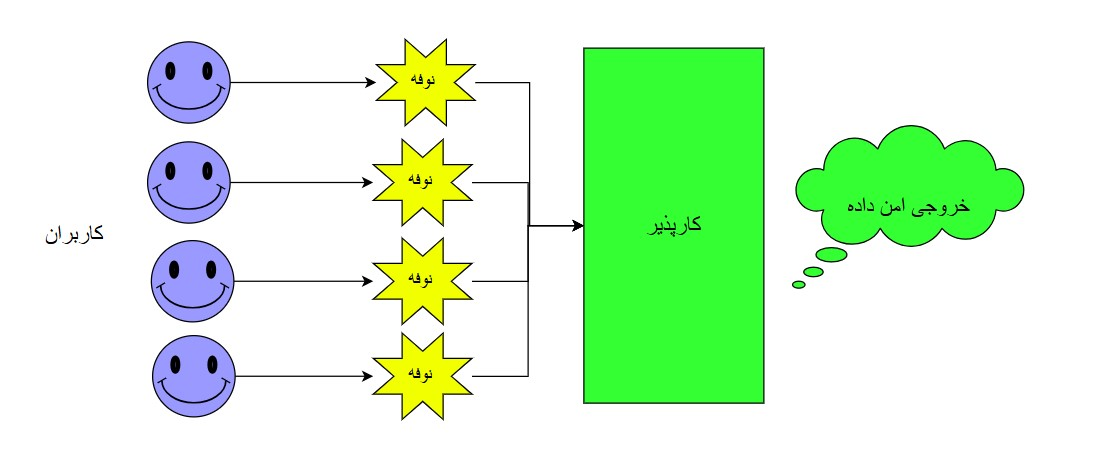
\includegraphics[width=0.9\textwidth]{figs/LDP.jpg}
  \caption{نحوه عملکرد حریم خصوصی تفاضلی محلی}
  \label{fig:LDP}
\end{figure}


\قسمت{حساسیت}

حساسیت\پانویس{Sensitivity} در زمینه حریم خصوصی داده‌ها به حداکثر تغییر در خروجی یک تابع به دلیل تغییر یک ورودی واحد اشاره دارد \مرجع{Dwork2011AFF}. به عبارت دیگر، حساسیت اندازه‌گیری می‌کند که چقدر می‌توان با تغییر یک ورودی، خروجی تابع را تحت تأثیر قرار داد. این ویژگی در طراحی سازوکار‌های حریم خصوصی تفاضلی محلی بسیار مهم است، زیرا تعیین می‌کند که چه مقدار نوفه باید به خروجی اضافه شود تا حریم خصوصی کاربران حفظ گردد.

\شروع{تعریف}[حساسیت]

حساسیت یک تابع $ f : \mathcal{X} \to \mathbb{R}^d$ به صورت زیر تعریف می‌شود:

\begin{equation}
\Delta f = \max_{x, x' \in \mathcal{X}} \|f(x) - f(x')\|
\end{equation}

\برچسب{تعریف: حساسیت}
\پایان{تعریف}


در عبارت بالا $\Delta f$ حساسیت تابع $f$ نامیده می‌شود و $\mathcal{X}$ دامنه ورودی ما است.

\قسمت{الگوریتم‌های حافظ حریم خصوصی تفاضلی}

\زیرقسمت{سازوکار لاپلاس}

سازوکار لاپلاس\پانویس{Laplace} در حریم خصوصی تفاضلی ایده‌ای ساده و در عین حال توانمند است. هرگاه بخواهیم آماری از داده‌ها مانند مجموع، میانگین و تعداد را منتشر کنیم، به‌جای پاسخ دقیق، همان پاسخ را با نوفه‌ای که از توزیع لاپلاس بدست می‌آید می‌فرستیم. مقدار پراکندگی این نوفه طوری تنظیم می‌شود که اگر اطلاعات یک فرد در پایگاه‌داده حذف یا اضافه شود، توزیع خروجی تقریباً تغییر نکند.  بدین‌ترتیب حضور یا عدم حضور آن فرد در نتیجه قابل تشخیص نیست. بزرگی نوفه به دو عامل بستگی دارد: حساسیت تابع و همچنین بودجهٔ حریم خصوصی. هرچه بودجه‌ی کمتری اختصاص دهیم حفاظت قوی‌تر شده و نوفه بیشتری اعمال می‌شود.

\شروع{تعریف}[سازوکار لاپلاس]

سازوکار لاپلاس روی یک تابع $ f : \mathcal{X} \to \mathbb{R}^d$ به صورت زیر تعریف می‌شود:

\begin{equation}
\mathcal{M}(D) = f(D) + \text{Lap}\left(\frac{\Delta f}{\epsilon}\right)
\end{equation}

\برچسب{تعریف: سازوکار لاپلاس}
\پایان{تعریف}

در عبارت بالا، ورودی مرکز یا $\mu$ در توزیع لاپلاس برابر صفر و همچنین ورودی مقیاس یا $b$ برابر $\frac{\Delta f}{\epsilon}$ در نظر گرفته شده است.


\زیرقسمت{سازوکار نمایی}

یکی از مشکلات سازوکار لاپلاس، عدم کارایی در مقادیر گسسته و غیر عددی است. از این رو سازوکار دیگری به نام سازوکار نمایی معرفی شد. این سازوکار چارچوبی فراهم می‌کند که در آن می‌توانیم تابع سودمنی دلخواه خود را تعریف کنیم. در واقع تابع $u$ هر ورودی و خروجی‌ تشکیل شده از پایگاه‌داده‌ی ما را به یک امتیاز سودمندی تبدیل می‌کند.

\begin{equation}
u : \mathbb{N}^{|X|} \times \mathcal{R} \rightarrow \mathbb{R}
\end{equation}

پس از محاسبه‌ی امتیاز هر خروجی، سازوکار گزینه‌ها را با احتمالی متناسب با توزیع نماییِ آن امتیاز انتخاب می‌کند. این انتخاب به‌گونه‌ای انجام می‌شود که گزینه‌های دارای امتیاز بالاتر، با احتمال بیشتری انتخاب شوند. این روش برای پرسش‌های غیرعددی (مثل «کدام محصول پرفروش‌تر است؟») بسیار سودمند خواهد بود. دقت کنید که ما اینجا نیاز به محاسبه حساسیت تابع سودمندی خود به شکل زیر داریم:

\begin{equation}
\Delta u = \max_{r \in \mathcal{R}} \max_{\substack{x,y \in \mathbb{N}^{|X|} \\ \|x - y\|_1 \leq 1}} |u(x,r) - u(y,r)|
\end{equation}

در نهایت سازوکار نمایی $\mathcal{M}_{E}(x,u,\mathcal{R})$ 
عنصر $r \in \mathcal{R}$ را با احتمالی متناسب با
$\exp\!\left(\frac{\varepsilon\,u(x,r)}{2\,\Delta u}\right)$
گزینش و اعلام می‌کند.

\زیرقسمت{پاسخ تصادفی}

پاسخ تصادفی روشی است که در نظرسنجی‌ها و جمع‌آوری داده‌های حساس کاربرد دارد. در این روش، به جای اینکه کاربر به‌طور مستقیم به یک سؤال پاسخ دهد، از یک سازوکار تصادفی استفاده می‌کند تا عدم قطعیت را به پاسخ خود اضافه کند. با اضافه کردن عدم قطعیت، مهاجم یا شخص متخاصم حتی اگر پاسخ نوفه‌دار شده‌ی کاربر را داشته‌باشد، نمی‌تواند با قطعیت جواب اصلی را مشخص کند. به بیان دیگر، کاربر با احتمال مشخصی پاسخ واقعی خود را ارائه می‌دهد و با احتمال دیگری پاسخ تصادفی دیگری را انتخاب می‌کند. این کار باعث می‌شود که احتمال شناسایی پاسخ واقعی کاربر کاهش یابد. مدل ریاضی پاسخ تصادفی توسط وارنر \مرجع{Warner1965RandomizedRA} معرفی شد.

\شروع{تعریف}[پاسخ تصادفی]

فرض کنید کاربر می‌خواهد به یک سؤال دودویی\پانویس{Binary} (بله/خیر) پاسخ دهد. اگر $x$ پاسخ واقعی کاربر باشد، سازوکار پاسخ تصادفی به صورت زیر عمل می‌کند:

\begin{equation}
\Pr[y = t] = 
\begin{cases} 
p, & \text{if} \quad t = x, \\[10pt]
1-p, & \text{if} \quad t \neq x
\end{cases}
\end{equation}

\برچسب{تعریف: پاسخ تصادفی}
\پایان{تعریف}

در عبارت بالا، $y$ پاسخ ارائه شده به سؤال است. $p$ احتمال اینکه کاربر پاسخ واقعی خود را ارائه دهد و $1{-}p$ احتمال این است که کاربر به طور تصادفی پاسخ مخالف را انتخاب کند. سازوکار پاسخ تصادفی اگر بخواهد $\epsilon{-}LDP$ باشد، باید مقدار $p$ را برابر $\frac{e^{\varepsilon}}{e^{\varepsilon}+1}$ قرار دهیم.

\زیرقسمت{پاسخ تصادفی عمومی}

پاسخ تصادفی به تنهایی جوابگوی مسائل پیچیده‌تر با دامنه بزرگتر نبود. پاسخ تصادفی عمومی\پانویس{Generalized Randomized Response}، شکل عمومی‌تر و انعطاف‌پذیرتر پاسخ تصادفی است \مرجع{Kairouz2016DiscreteDE, Kairouz2014ExtremalMF}. این الگوریتم را به اختصار، «جی آر آر» می‌نامند.

\شروع{تعریف}[پاسخ تصادفی عمومی]

فرض کنید کاربر می‌خواهد به یک سؤال با $k$ گزینه پاسخ دهد. اگر $x$ پاسخ واقعی کاربر باشد، سازوکار پاسخ تصادفی عمومی به صورت زیر عمل می‌کند:

\begin{equation}
\Pr[y = t] = 
\begin{cases} 
p, & \text{if} \quad t = x, \\[10pt]
\frac{1 - p}{k - 1}, & \text{if} \quad t \neq x
\end{cases}
\label{equ:GRR}
\end{equation}

\برچسب{تعریف: پاسخ تصادفی عمومی}
\پایان{تعریف}

سازوکار پاسخ تصادفی اگر بخواهد $\epsilon{-}LDP$ باشد، باید مقدار $p$ را برابر $\frac{e^{\varepsilon}}{e^{\varepsilon}+k-1}$ قرار دهیم.

پژوهش آرکولزی و همکاران \مرجع{Arcolezi2023RevealingTT} یک چارچوب نرم‌افزاری را برای حسابرسی و ارزیابی عملی پروتکل‌های حریم خصوصی تفاضلی محلی معرفی می‌کند. در نتیجه آزمایشات این پژوهش، پاسخ تصادفی عمومی بهترین عملکرد را داشته است. به بیان دیگر اتلاف حریم خصوصی که به صورت عملی برای پاسخ تصادفی عمومی اندازه‌گیری شد، بسیار نزدیک به تضمین نظری آن بوده است. یعنی این سازوکار دقیقاً همان سطحی از حریم خصوصی را که ادعا می‌کند، در عمل نیز ارائه می‌دهد و بیش از حد محافظه‌کارانه عمل نمی‌کند. دلیل این امر، سادگی آن و عدم وجود مراحل کدگذاری پیچیده است که باعث از دست رفتن اطلاعات نمی‌شود.

\زیرقسمت{الگوریتم تصادفی‌سازی متقارن}

به الگوریتم‌هایی که در فرآیند تصادفی‌سازی برای حفظ حریم خصوصی کاربران، احتمال حفظ مقدار اصلی داده‌ها برابر با احتمال تغییر آن‌ها باشد، متقارن می‌گوییم. به عنوان مثال در مسائلی که ورودی با دامنه دودویی دارند، احتمال زیر برقرار است:

\begin{equation}
Pr[y = 1 | x = 1] = Pr[y = 0 | x = 0] 
\end{equation}

در عبارت بالا، $x$ ورودی و $y$ خروجی الگوریتم است.

\قسمت{ترکیب متوالی}

در زمینه حریم خصوصی، ترکیب متوالی\پانویس{Sequential Composition} به این صورت تعریف می‌شود که اگر شما چندین سازوکار تصادفی را به‌طور متوالی روی یک مجموعه داده اجرا کنید، حریم خصوصی شما به‌طور کلی نقض می‌شود. حتی اگر هر یک از این سازوکار‌ها جداگانه ایمن باشند، در نهایت نمی‌توانید حریم خصوصی را تضمین کنید \مرجع{nissim2012approximately}. این اصل ساده اما سرنوشت‌ساز، طراحان الگوریتم‌های حریم خصوصی را مجبور می‌کند بودجهٔ حریم خصوصی را میان سازوکارهای مختلف تقسیم کنند. از آنجایی که بوجه‌ی حریم خصوصی محدود است، اگر تعداد سازوکارهای مختلف زیاد باشد، بودجه‌ی کمی به هر کدام می‌رسد و به سبب آن سودمندی الگوریتم کاهش میابد.

به بیان ریاضی، پس از اجرای $k$ سازوکار مستقل روی یک مجموعه داده که هرکدام $\epsilon{-}LDP$ هستند، می‌توان گفت الگوریتم کلی ما با بودجه‌ای برابر با مجموع تمام بودجه‌ها، حریم خصوصی تفاضلی را ارضا می‌کند:

$$\mathcal{M}_i(x) \quad satisfies \quad \epsilon_i{-}LDP$$
$$\mathcal{M} = \{ \mathcal{M}_1 , \mathcal{M}_2 , ... , \mathcal{M}_m \} \quad satisfies \quad \sum_{i=1}^{m} \epsilon_i{-}LDP$$

در سامانه‌هایی که پرس‌و‌جو‌های\پانویس{Query} متعدد روی یک معیار داریم (مانند دریافت میزان مصرف باتری هر یک ساعت یکبار)، هر بار باید روی یک داده نوفه اعمال کنیم و به سمت کارپذیر بفرستیم. گرچه مقدار خام داده ممکن است هر بار تغییر کند، ولی چون از یک جنس است و مربوط به یک معیار می‌شود، قانون ترکیب متوالی روی آن صدق می‌کند. بودجه‌ی حریم خصوصی بین تعداد استفاده از سازوکار تصادفی‌سازی تقسیم شده و سودمندی کاهش میابد.

شایان ذکر است که در داده‌های با ابعاد بالا نیز، با چالش ترکیب متوالی روبه‌رو هستیم. در داده‌های با ابعاد بالا، احتمال وجود وابستگی میان ابعاد زیاد می‌شود (مانند ارتباط مستقیم بین سن و میزان درآمد). زمانیکه سازوکارهای تصادفی‌سازی را روی ابعاد وابسته به هم اعمال می‌کنیم، مانند این است که به یک مجموعه داده نوفه تزریق می‌کنیم. از این رو شامل قانون ترکیب متوالی شده و بوجه‌ی حریم خصوصی بین سازوکارها تقسیم می‌شود.

\قسمت{ترکیب موازی}

در ترکیب موازی\پانویس{Parallel Composition}، الگوریتم‌های مختلف حریم خصوصی تفاضلی به طور همزمان روی یک یا چند پایگاه‌داده مجزا  از یکدیگر اعمال می‌شوند \مرجع{mcsherry2009privacy}. در این حالت، بودجه‌ی الگوریتم کلی برابر با حداکثر بودجه‌ی الگوریتم‌هاست:

$$\mathcal{M}_i(x) \quad satisfies \quad \epsilon_i{-}LDP$$
$$ \mathcal{M} = \{ \mathcal{M}_1 , \mathcal{M}_2 , ... , \mathcal{M}_m \} \quad satisfies \quad \max \{ \epsilon_1 , \epsilon_2 , ... , \epsilon_m \}{-}LDP$$

\قسمت{روش‌های کدگذاری}

هر کاربر به منظور ارسال داده‌ها سمت کارپذیر، باید ابتدا اطلاعات خود را در فرمت خاصی کدگذاری\پانویس{Encode} کند. اینکار به دو دلیل نیاز است:

\شروع{شمارش}
\فقره افزایش سرعت ارسال پیام
\فقره بهبود فرایند تصادفی‌سازی
\پایان{شمارش}

\زیرقسمت{کدگذاری مستفیم}

کدگذاری مستقیم\پانویس{Direct Encoding} یکی از روش‌های ساده برای کدگذاری مقادیر ورودی در پروتکل‌های حفاظت از حریم خصوصی محلی است. در این روش، داده‌ی هر کاربر بدون هیچ‌گونه تبدیل اولیه مستقیماً به عنوان خروجی کدگذاری‌شده و ارسال می‌شود. این روش برای مواردی که دامنه داده‌ها کوچک است (مانند داده‌های طبقه‌بندی‌شده یا مقادیر گسسته محدود) مناسب‌تر خواهد بود. این کدگذاری در پژوهش \مرجع{Wang2016PrivateWH} استفاده شده است.

\begin{equation}
 v = Encode(v)
\end{equation}

برای تصادفی‌سازی در این کدگذاری، باید از سازوکار تصادفی‌سازی عمومی استفاده کرد. دقت کنید که کارایی و عملکرد این روش با افزایش دامنه، به شدت کاهش میابد. از آنجایی که در الگوریتم تصادفی‌سازی عمومی، مقدار $p$ برابر $\frac{e^{\varepsilon}}{e^{\varepsilon}+k-1}$ است، با افزایش دامنه یا همان $k$، احتمال انتخاب شدن مقدار اصلی در تصادفی‌سازی کاهش یافته و به سبب آن، سودمندی دلخواه بدست نمی‌آید. همچنین یکی دیگر از معایب این روش، هزینه‌ی ارتباطی\پانویس{Communication Cost} بالا است.

\زیرقسمت{کدگذاری یکانی}

کدگذاری یکانی\پانویس{Unary Encoding} یکی از روش‌های متداول برای کدگذاری مقادیر ورودی در پروتکل‌های حفاظت از حریم خصوصی تفاضلی محلی است. در این روش، هر مقدار ورودی به یک بردار دودویی با طول ثابت تبدیل می‌شود. تنها یک بیت از این بردار که نماینده ورودی است، مقدار 1 دارد و بقیه بیت‌ها 0 هستند.

\begin{equation}
Encode(v) = [0, \text{···} ,0,1,0, \text{···} , 0], \quad \text{\lr{only the v-th position is 1}}
\end{equation}

به منظور تصادفی‌سازی از فرمول زیر استفاده می‌کنیم. $p$ احتمال 1 شدن بیتی است که قبلا مقدار 1 داشته است. همچنین $q$ احتمال 1 شدن بیتی است که قبلا مقدار 0 داشته است:

\begin{equation}
\Pr[y = 1] =
\begin{cases} 
p, & \text{if} \quad x = 1, \\[10pt]
q, & \text{if} \quad x = 0.
\end{cases}
\end{equation}

اگر شرط زیر برقرار باشد، می‌توان گفت پروتکل کدگذاری یکانی، حریم خصوصی تفاضلی را ارضا کرده است:


\begin{equation}
\epsilon = \ln \left( \frac{p(1 - q)}{(1 - p)q} \right)
\label{equ:unary}
\end{equation}

\زیرقسمت{کدگذاری یکانی متقارن}

پروتکل کدگذاری یکانی متقارن\پانویس{Symmetric Unary Encoding} به این صورت تعریف می‌شود که حاصل جمع مقادیر احتمال $p$ و $q$ برابر 1 باشد:
$$p + q = 1$$
با توجه به قاعده \رجوع{equ:unary}، مقادیر $p$ و $q$ به صورت زیر بدست می‌آیند:

$$p = \frac{e^{\epsilon/2}}{e^{\epsilon/2} + 1}, \quad q = \frac{1}{e^{\epsilon/2} + 1}$$

\زیرقسمت{درهم‌سازی محلی}

در پروتکل کدگذاری یکانی، هزینه‌ی ارتباطی به صورت خطی با زیاد شدن دامنه‌ی ورودی، افزایش میابد. این افزایش هزینه در بعضی برنامه‌های کاربردی موجب بروز تاخیر بسیار زیاد در عملکرد سامانه می‌شود. بنابراین به پروتکل دیگری نیاز داریم که بزرگ شدن دامنه‌ی ورودی، تاثیر چندانی در هزینه ارتباطی نداشته باشد.

ایده‌ی اولیه این است که از یک تابع درهم‌ساز\پانویس{Hash Function} استفاده کرده و اندازه‌ دامنه‌ی ورودی را کاهش دهیم. این ایده مشکل تصادم\پانویس{Collision} را به همراه دارد. به بیان دیگر، دو ورودی به یک خروجی تبدیل شده و در زمان کدگشایی\پانویس{Decode} نمی‌توان مقدار درست ورودی را بدست آورد. در پژوهش رپور \مرجع{erlingsson2014rappor} چندین راه برای حل این مشکل ارائه شده است:

\شروع{شمارش}
\فقره استفاده از چند تابع درهم‌ساز به منظور کاهش احتمال تصادم
\فقره استفاده از مفهوم گروه\پانویس{Cohort} که در آن هر گروه دارای مجموعه‌ای از توابع درهم‌ساز خواهد بود.
\پایان{شمارش}

البته با توجه به روش‌های مذکور، نمی‌توان به صورت قطعی مشکل تصادم را حل کرد و این مشکل در کاهش سودمندی تأثیر می‌گذارد. روش بهتر این است که هر کاربر توابع درهم‌ساز محلی خود را داشته باشد. به این روش، درهم‌ساز محلی\پانویس{Local Hashing} می‌گوییم. این روش به صورت کارا در الگوریتم‌های حفظ حریم خصوصی تفاضلی محلی استفاده می‌شود. کاربران با کمک توابع درهم‌ساز، ابتدا دامنه‌ی داده‌های خود را کاهش داده، تصادفی‌سازی کرده و در نهایت به سمت کارپذیر ارسال می‌کنند. در ادامه تعریف درهم‌ساز محلی دودویی را ارائه می‌دهیم:

\شروع{تعریف}[درهم‌ساز محلی دودویی]

فرض کنید $\mathbb{H}$ یک خانواده جهانی از توابع درهم‌ساز باشد. هر تابع درهم‌ساز $H \in \mathbb{H}$، یک ورودی با دامنه‌ی $d$ را به یک عدد تک بیتی تبدیل می‌کند. شرطی روی این خانواده از توابع درهم‌ساز اعمال می‌شود به صورت زیر خواهد بود:

\begin{equation}
\forall x, y \in [d], x \neq y : \Pr_{H \in \mathbb{H}} [H(x) = H(y)] \leq \frac{1}{2}
\end{equation}

\برچسب{تعریف: درهم‌ساز محلی دودویی}
\پایان{تعریف}

به منظور تصادفی‌سازی از فرمول زیر استفاده می‌کنیم:

$$\text{Perturb}_{\text{BLH}}(\langle H, b \rangle) = \langle H, b' \rangle, \quad \Pr[b' = 1] = 
\begin{cases} 
p = \dfrac{e^\epsilon}{e^{\epsilon}+1}, & \text{if} \quad b = 1 \\ 
q = \dfrac{1}{e^{\epsilon}+1}, & \text{if} \quad b = 0 
\end{cases}$$

\زیرقسمت{بلوم فیلتر}

بلوم‌فیلتر\پانویس{Bloom Filter} یک ساختار داده‌ای است که هدف اصلی آن انجام عملیات بررسی عضویت (یعنی تعیین اینکه یک عنصر در مجموعه‌ای وجود دارد یا خیر) با استفاده حداقلی از حافظه است. این فیلتر به ما کمک می‌کند تا سریعاً امکان وجود یک عنصر را بدون نیاز به ذخیره کل مجموعه در حافظه تشخیص دهیم.

فرض کنید آرایه‌ای از بیت‌ها (معمولاً همه صفر) و چند تابع درهم‌ساز داریم. مطابق شکل \رجوع{fig:BloomFilter} زمان درج هر عنصرِ جدید، آن را با همه توابع درهم‌سازی کرده و مقدار 1 برای بیت‌های متناظر درنظر گرفته می‌شود. دقت کنید که ممکن است درهم‌سازی توابع، تصادم داشته باشد و چند بیت 1 روی هم بیفتند. هنگام پرس‌وجوی عنصر،  دوباره باید با همه‌ی توابع درهم‌سازی شود و اگر همه‌ی بیت‌های متناظر یک باشند، می‌گوییم این عنصر احتمالاً در آرایه وجود دارد. حتی اگر یکی صفر باشد قطعاً عنصر مورد نظر در آرایه وجود ندارد. با تنظیم اندازهٔ آرایه و تعداد توابع هش، می‌توان احتمال خطا را به دلخواه کم کرد. از همین ویژگی در پژوهش رپور نیز بهره گرفته شده تا رشته‌های دلخواه کاربران به‌صورت فشرده و بی‌نیاز از فهرست پیش‌تعریف‌شده گزارش شود و حریم خصوصی حفظ گردد.

بلوم فیلتر در بسیاری از سیستم‌ها و سرویس‌ها استفاده می‌شود از جمله:

\شروع{فقرات}
\فقره گوگل کروم: برای ویژگی مرور امن\پانویس{Safe Browsing} از بلوم فیلتر استفاده می‌شود تا به سرعت خطرناک بودن آدرس‌های اینترنتی را بررسی کند.
\فقره مدیُم\پانویس{Medium}: از بلوم فیلتر برای جلوگیری از نمایش پست‌هایی که کاربر قبلاً دیده است، استفاده می‌کند.
\فقره کساندرا\پانویس{Cassandra} و اچ بیس\پانویس{HBase}: برای بهینه‌سازی جستجوی داده‌ها در جدول‌های ذخیره‌شده در دیسک استفاده می‌شود.
\فقره آکامای\پانویس{Akamai}: در سرویس‌های حافظه نهان\پانویس{Cache} خود برای بهبود سرعت و کارایی تحویل محتوا از بلوم فیلتر استفاده می‌کند.
\پایان{فقرات}

\begin{figure}[h]
  \centering
  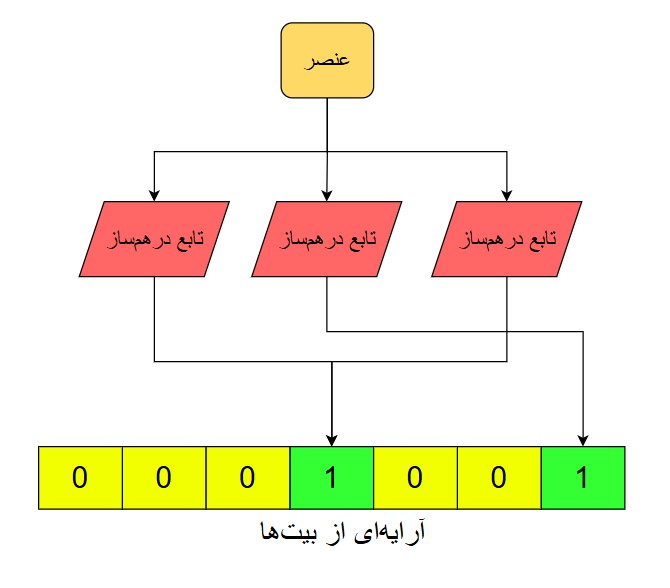
\includegraphics[width=0.9\textwidth]{figs/BloomFilter.jpg}
  \caption{شیوه‌ی درج عنصر با استفاده از بلوم فیلتر}
  \label{fig:BloomFilter}
\end{figure}


